\chapter{级数}
\label{ch:Series}

\section*{学习目标}
\begin{todolist}
	\item 绘制\gls{pascaltri}
	\item 掌握\gls{factorial}的求算
	\item 掌握\gls{combi}的求算
	\item 牢记并运用$(a+b)^n$的展开式结果
	\item 确定\gls{dcsl},\gls{commondiff},\gls{generalterm}和$n$项和公式,并用于解决问题
	\item 确定\gls{dbsl},\gls{commonratio},\gls{generalterm}和$n$项和公式,并用于解决问题
	\item 明确等比数列\gls{converge}的条件,以及无穷级数之和
\end{todolist}
\clearpage

\section{组合数}
\label{sec:Combination}
学习这一张需要先把多项式乘法的基础打好

\subsection*{杨辉三角}
\label{subsec:Pascal's Triangle}
打开$(a+b)^2$得到$\boxed{1}a^2+\boxed{2}ab+\boxed{1}b^2$。打开$(a+b)^3$得到$\boxed{1}a^3+\boxed{3}a^2b+\boxed{3}ab^2+\boxed{1}b^3$。如果持续打开这样的结果,把每一项的系数写下来会得到这样的排布特征:
\begin{figure}[H]
\centering
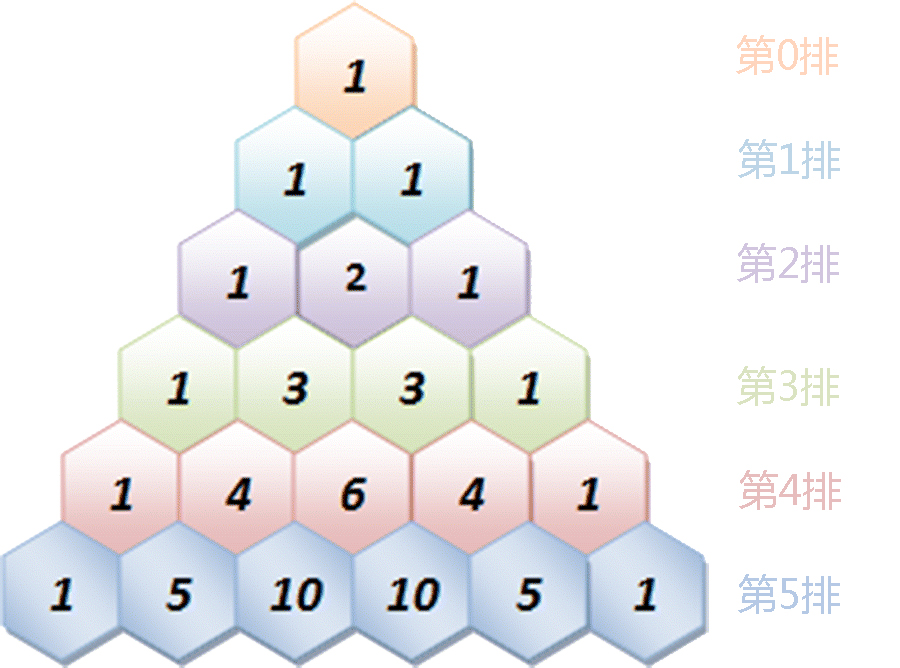
\includegraphics[width=0.6\textwidth]{pacal's triangle}
\caption{杨辉三角、帕斯卡三角的前$5$排,最上方的单独的数字$1$算做第$0$排。}
\end{figure}

\begin{SummBox}
\noindent 杨辉三角的第$n$排会有$n+1$个数字;\\
杨辉三角的每一排数字都是关于中轴线对称;\\
每一排的最左边和最右边数字都是$1$;\\
\textbf{每一排的数字都是通过上一排与之相邻的两个数字相加而产生的。}
\end{SummBox}

\subsection*{阶乘}
\label{subsec:Factorial}
定义$n!$为这样的运算:
\[
	n!=n\times (n-1)\times(n-2)\times(n-3)\times \ldots \times 2\times 1 
\]
把这种运算称之为\gls{factorial},其中根据阶乘的性质推导,我们定义$0!=1$


\subsection*{组合}
定义Combination的运算如下:
\[
	nCr={n\choose r}=\frac{n!}{(n-r)!\times r!}=\frac{n\times(n-1)\times \cdots \times(n+1-r)}{r\times (r-1)\times \cdots \times 2\times 1}
\]
其计算结果代表\emph{从$n$个物体当中,挑选$r$个物体,且无需考虑物体取出的顺序,总共可行的挑选方案个数}

\begin{TaskBox}
求算${5\choose 3}$的结果,并描述一个场景以该结果做为答案。
\end{TaskBox}

组合数还具有如下的几个常见性质:
\begin{align*}
{n\choose 0} &= {n\choose n}=1\\
{n\choose r} &= {n\choose n-r}\\
{n\choose 0}+{n\choose 1} &+{n\choose 2}+\cdots +{n\choose n}=2^n
\end{align*}
这些性质都可以通过定义去证明,尝试一下吧。
\clearpage


\section{二项展开式}
\label{sec:Binomial Expansion}
形如$(\Box+\triangle)^n$的表达式被称之为\gls{binomial}。当我们对这样的表达式进行打开的时候,可以利用杨辉三角作为系数加快自己的展开过程。

\begin{ExampleBox}
展开$(x+1)^5$
\tcblower
杨辉三角的第五排是$1,5,10,10,5,1$作为系数,并且进行降次排列得到\\
$(x+1)^5=1x^5+5x^4\times1+10x^3\times 1^2+10x^2\times 1^3+5x\times1^4+1\times 1^5$
\end{ExampleBox}

有没有发现:${5\choose 3}=10$ 刚好就是杨辉三角的第\emph{五}排,第\emph{四}个数字。所以如果需要展开一个更为复杂的二项式,比如$(a+b)^{100}$。则无需再绘制$100$行的杨辉三角了,可以直接用组合数来进行替代。因此$(a+b)^{100}={100\choose 0}a^{100}b^0+{100\choose 1}a^{99}b^1+{100\choose 2}a^{98}b^2+\cdots + {100\choose 99}a^1b^{99}+ {100\choose 100}a^0 b^{100}$

这样就可以得到最重要的二项展开式定理:
\begin{align*}
	(a+b)^n &={n\choose 0}a^{n}b^0+{n\choose 1}a^{n-1}b^1+\cdots + {n\choose n-1}a^1b^{n-1}+ {n\choose n}a^0 b^{n}\\
	        &=\sum_{k=0}^{n}{n\choose k}a^{n-k}b^k
\end{align*}
\clearpage

\section{等差数列}
\label{sec:Arithmetic Progression}
数列是有顺序的数字排列,比如杨辉三角的每一行都可以当成是一个含有$n+1$个数字的数列;当一个数列的后一项与前一项相差为恒定值的时候,这种数列被称之为\gls{dcsl}

比如:
\begin{align*}
1\quad 3\quad 5\quad 7 \  \ldots \\
10\quad 7 \quad 4\quad 1 \ \ldots \\
\sqrt 2 \quad 2\sqrt2 \quad 3\sqrt2 \ \ldots
\end{align*}

\subsection*{公差与通项公式}
\label{subsec:Common Difference and General Term}
在一个等差数列中,后一项与前一项之差为$u_{n+1}-u_{n}$或者是$u_{n}-u_{n-1}$,一般计作$d$,称之为公差。是可正可负,也可以为0的。

因此描述任意一项的数值的公式——\gls{generalterm}就可以如下的关系表示:
\[
	u_n=a+(n-1)\cdot d
\]
其中,\\
$u_n$表示数列当中的第$n$项\\
$a$是该等差数列的第一项\\
$d$是公差

\begin{TaskBox}
尝试写出三个等差数列的通项公式
\end{TaskBox}


\subsection*{等差数列的求和公式}
\label{Sum of Arithmetic}
数学王子\href{https://en.wikipedia.org/wiki/Carl_Friedrich_Gauss#Algebra}{高斯}在7岁的时候就研究出了等差数列的求和公式:
\begin{align*}
	S_n &= \frac{u_1+u_n}{2}\cdot n\\
	    &=na+\frac{1}{2}n(n-1)d
\end{align*}

\begin{TaskBox}
不准使用计算器,求算$1+2+3+\cdots +99 +100$。
\end{TaskBox}
\clearpage


\section{等比数列}
\label{sec:Geometric Progression}
当后一项与前一项的比值恒定时,具有这种特征的数列被称之为\gls{dbsl}。

比如:
\begin{align*}
1\quad 3\quad 9\quad 27 \  \ldots \\
1024\quad 512 \quad 256\quad 128 \ \ldots \\
\sqrt 2 \quad 2 \quad 2\sqrt2 \ \ldots
\end{align*}

\subsection*{公比与通项公式}
\label{subsec:Common Ratio and General Term}
等比数列中,后一项与前一项之比$\frac{u_{n+1}}{u_n}$或者$\frac{u_{n}}{u_{n_1}}$称之为公比,计作$r$。

因此求算等比数列的\gls{generalterm}的公式为:
\[
	u_n=a\cdot r^{(n-1)}
\]

\begin{TaskBox}
试写出以上三个等比数列的公比和通项公式
\end{TaskBox}


\subsection*{求和公式}
等比数列的求和公式推导难度并不大,仅需要把每一个元素都乘上公比,进行\href{https://www.cuemath.com/algebra/sum-of-a-gp/}{错位相消即可}。
最终得到:
\[
	S_n=\frac{a(1-r^n)}{1-r}
\]
该公式是当公比$r\neq1$时采用的,如果$r=1$,则意味着该等比数列是个固定值数列,每一项都和第一项相等$u_n=u_1=a$。因此$S_n=n\cdot a$即可。

\subsection*{等比数列的收敛性}
\label{subsec:Convergence of GP}
当公比小于1时,等比数列越来越小,而其前$n$项和会越来越逼近于一个恒定值,这种特性叫做\gls{converge}。是研究数列的一个重要性质。

\begin{TaskBox}
查看\href{https://www.bilibili.com/video/BV1eJ411z78q}{cigar666}的视频,并描述当公比分为为$\frac{1}{4}$,$\frac{1}{5}$时。等比数列的求和会逼近哪一个值?
\end{TaskBox}

实际上,这个问题从通项公式就可以回答了。
\begin{align*}
S_n &= \frac{a(1-r^n)}{1-r}\\
 	&=\frac{a}{1-r} \cdot (1-r^n)
\end{align*}

前面的部分$\frac{a}{1-r}$为恒定值。而当$|r|<1$时,由于指数的运算的性质,当$n$是一个非常大数字时,$r^n\to 0$。因此此时我们计作无穷多项和Sum to Infinity
\[
	S_{\infty} = \frac{a}{1-r}  \quad \text{when } |r|<1
\]